\chapter{Fundamentação Teórica}
\label{cap:fundamentacao-teorica}


\section{Os Gêneros dos Jogos}
\label{sec:os-generos-dos-jogos}

Gênero de jogo pode ser definido como uma modalidade ou tipo que permite o agrupamento de diversos jogos de acordo com suas características de jogabilidade.
Segundo Eucidio, pensar no jogo é pensar no estilo de produção que o jogo seguirá, pensar nos desafios, dificuldades e possibilidades.
A plataforma dos jogos também influenciam para determinar o gênero do jogo. Em smartphones, por exemplo, os jogos tendem a ser mais casuais e rápidos. Existe uma infinidade de categorizações, abaixo encontra-se listadas alguma das mais populares. 

\begin{alineascomponto}
\item Jogos de Ação\\
Significa atividade, agir de acordo com  situação. O jogador tem que tomar alguma ação em tempo real, agindo rapidamente. Jogos deste gênero é o mais popular para a plataforma PC. Um exemplo de jogo de ação é o Half-Life 2, onde possui as características de ser um jogo sagaz, envolvente e com enredo, na figura 4 encontra-se a capa da Mídia digital deste jogo.
\end{alineascomponto}
\begin{figure}[h!]
		\centering
		\Caption{\label{fig:exemplo-4}Jogo Half Life 2, desenvolvido pela Valve Corporation(2004)}	
		\UECEfig{}{
			\fbox{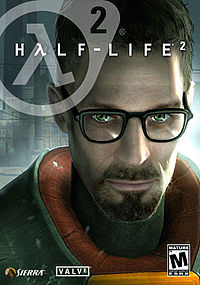
\includegraphics[width=5cm]{figuras/HalfLife}}
		}{
			\Fonte{http://www.ign.com/games/half-life-2/pc-492830, 2004}			
		}	
	\end{figure}
\begin{alineascomponto}
\item Jogos de Simulação\\
É a representação da realidade, são jogos que simulam situações vividas por seres humanos. A principal utilização por este gênero é para simulação de voos, tendo como objetivo o treinamento de pilotos como por exemplo o jogo FlightSimulator da Microsoft. Na figura 5 é possível ver a simulação que ocorre no jogo.
\end{alineascomponto}
\begin{figure}[h!]
		\centering
		\Caption{\label{fig:exemplo-5}Jogo Flight Simulator desenvolvido pela Microsoft (2015)}	
		\UECEfig{}{
			\fbox{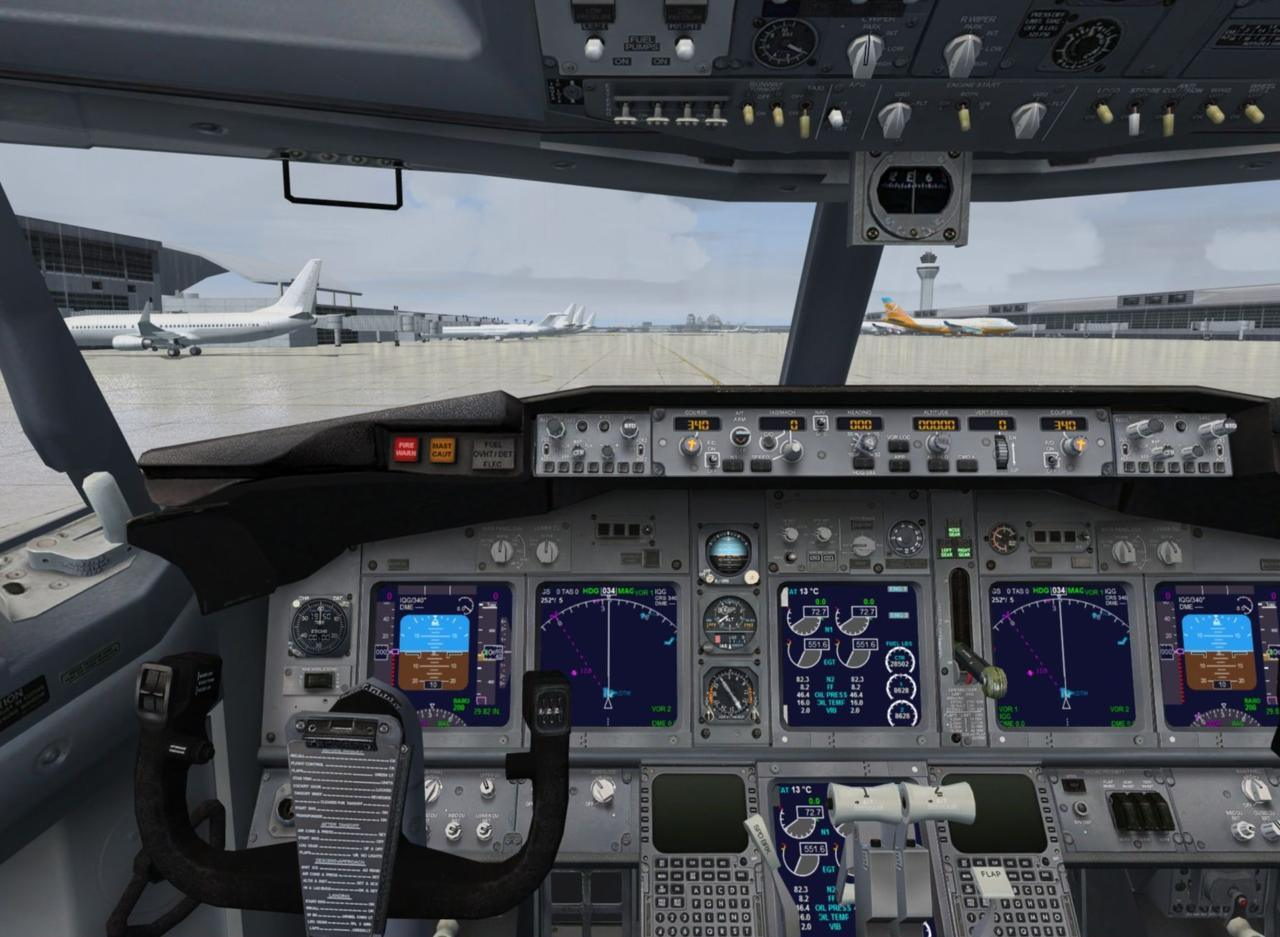
\includegraphics[width=7cm]{figuras/MFS}}
		}{
			\Fonte{http://microsoft-news.com/microsoft-licenses-flight-simulator-game-franchise-to-dovetail-games-new-game-coming-in-2015/, 2014}			
		}	
	\end{figure}

\begin{alineascomponto}
\item Jogos de RPG\\
Tem como característica o desenvolvimento gradativo do personagem. O jogador assume o papel do personagem aonde pode haver narrativas para auxiliar no decorrer do jogo.
Um jogo muito conhecido que que utiliza deste gênero é o Final Fantasy XIII,  na figura 6 encontra-se a capa da Mídia digital deste jogo.
\end{alineascomponto}

\begin{figure}[h!]
		\centering
		\Caption{\label{fig:exemplo-6}Jogo Final Fantasy XIII desenvolvido pela Square Enix (2009)}	
		\UECEfig{}{
			\fbox{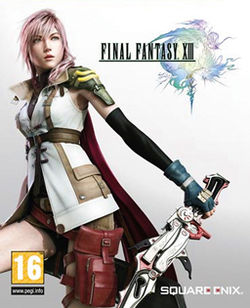
\includegraphics[width=7cm]{figuras/FF}}
		}{
			\Fonte{http://www.ffotaku.com/final-fantasy-xiii/wallpapers.php}			
		}	
	\end{figure}
	
\begin{alineascomponto}
\item Jogos de Esportes\\
A principal caracterıstica de jogos deste gênero é o controle ocorre sobre o personagem não mecânico. Normalmente o jogo tem um esforço fısico do jogador no
mundo virtual, em alguns jogos o personagem cansa e diminui sua velocidade. Um exemplo de jogo de esporte é o FIFA, conforme demostrado na figura 7.
\end{alineascomponto}
\begin{figure}[h!]
		\centering
		\Caption{\label{fig:exemplo-7}Fifa 15 desenvolvido pela EA Sports (2014)}	
		\UECEfig{}{
			\fbox{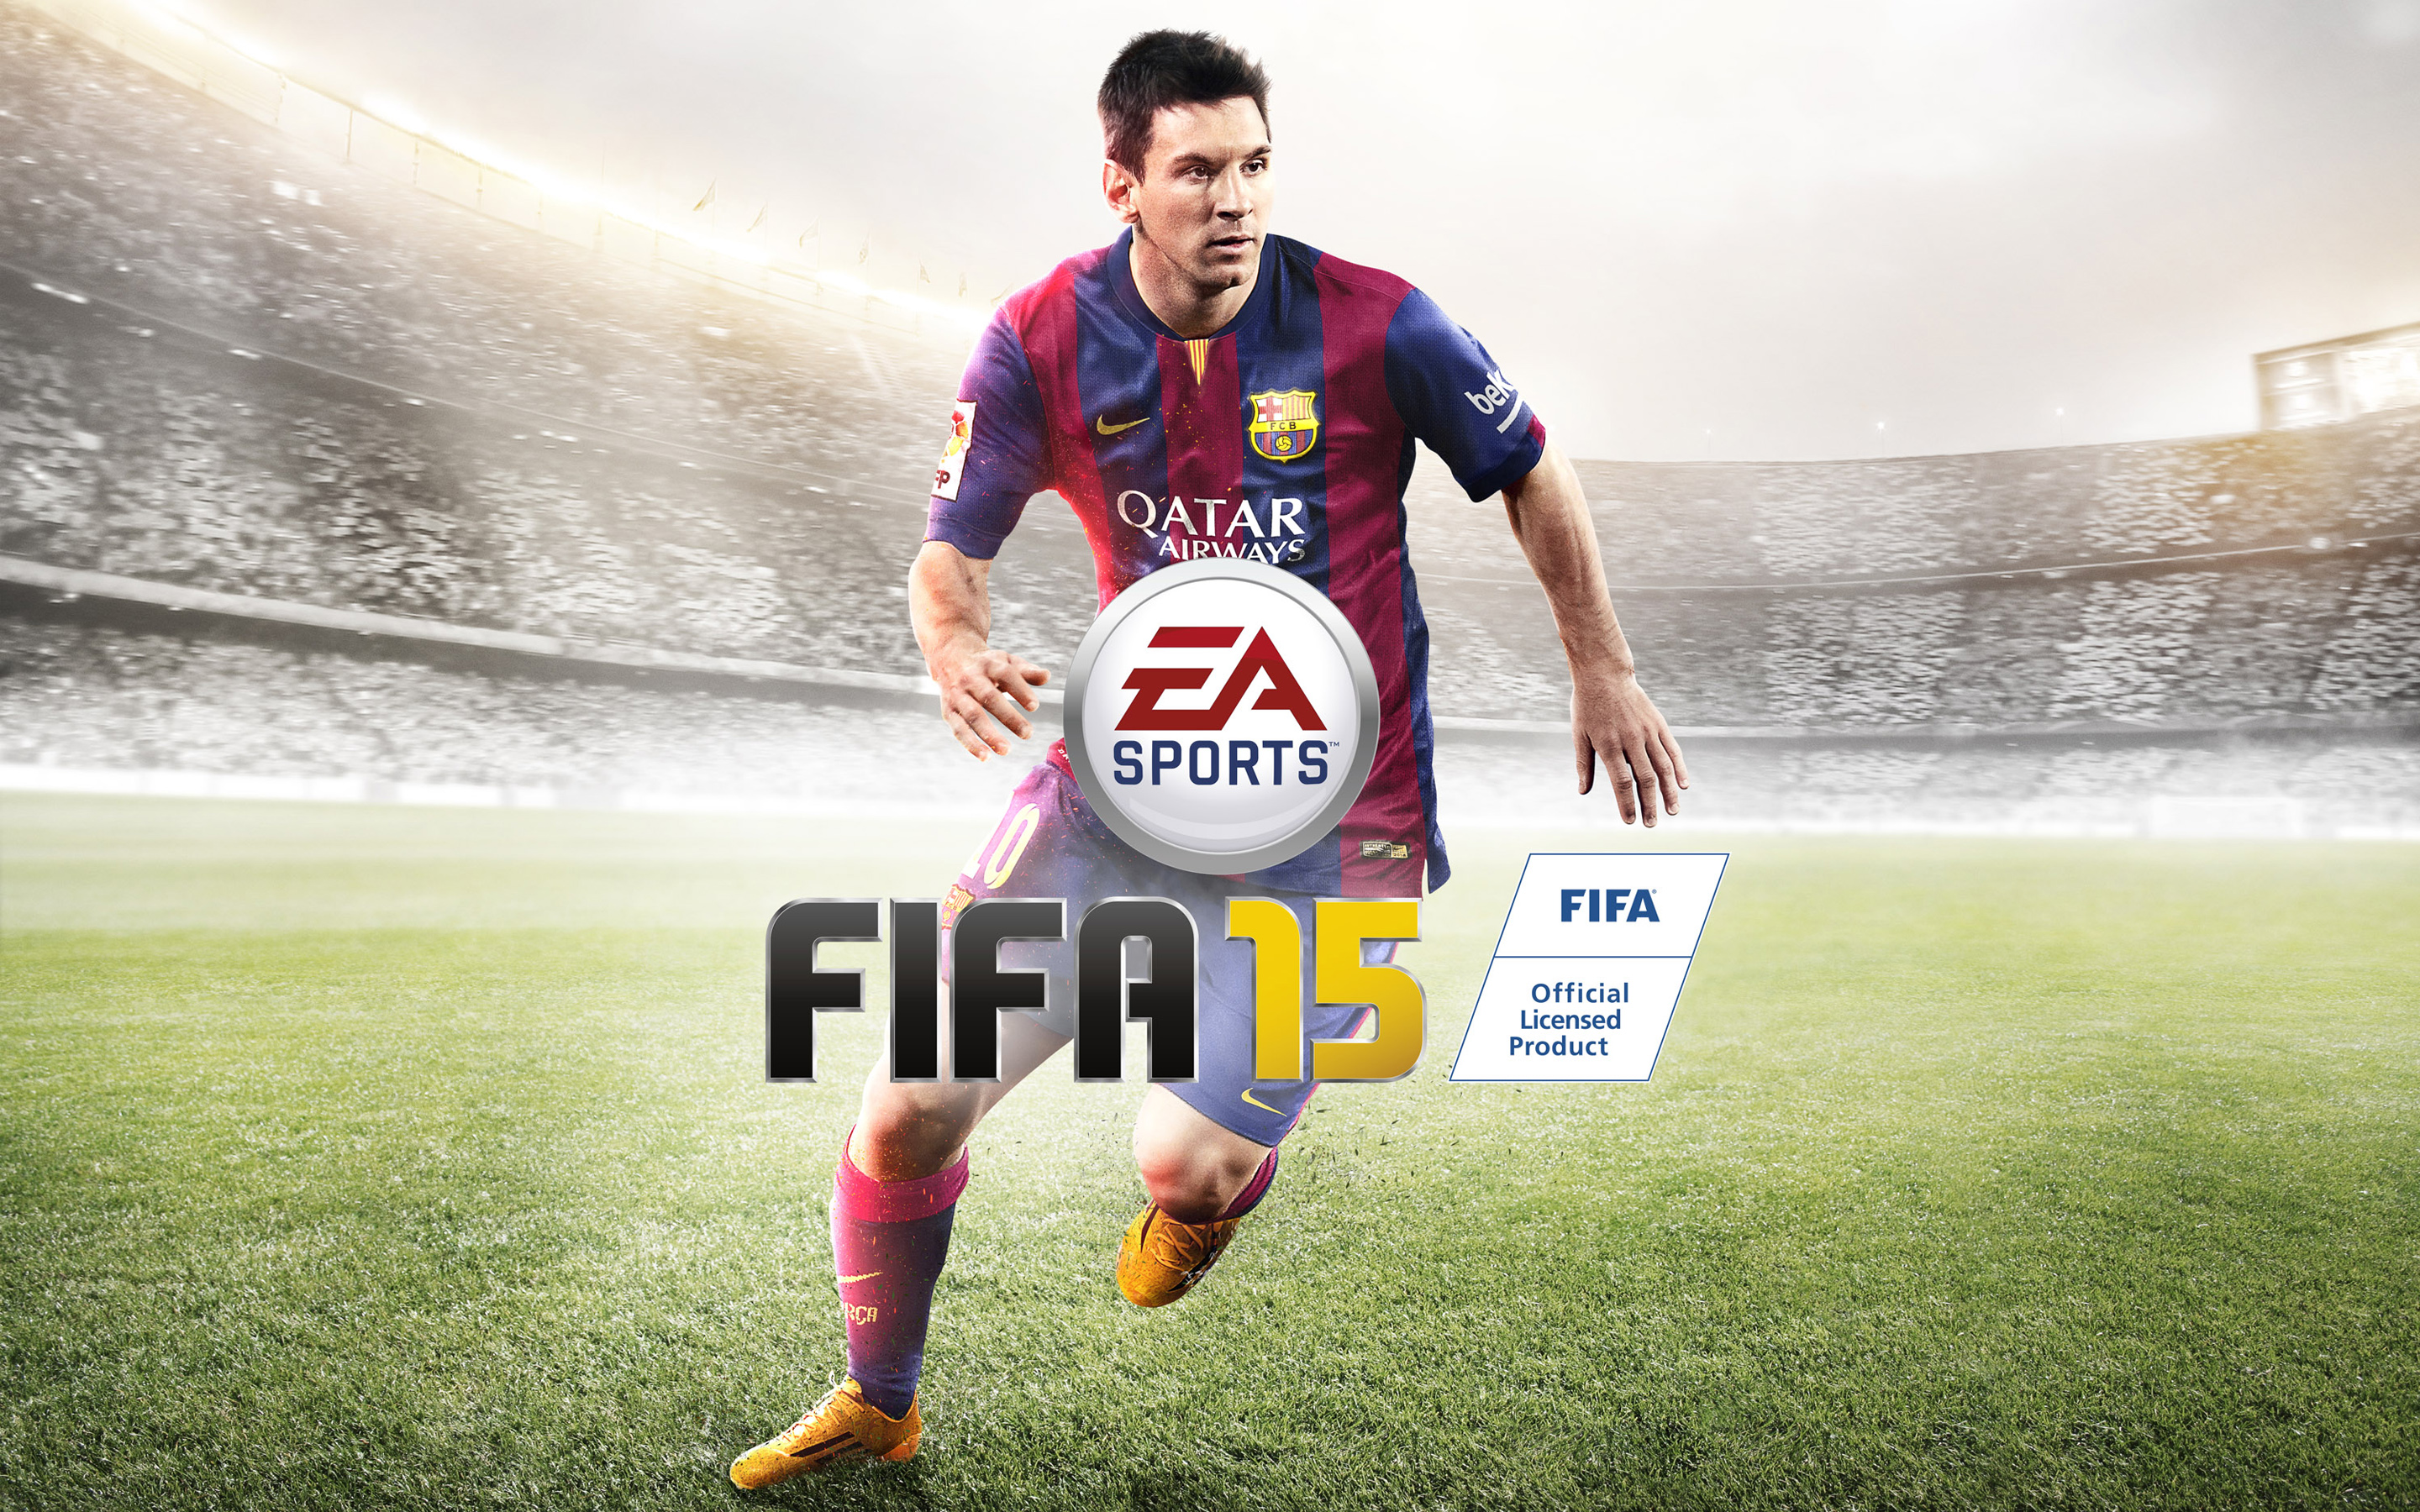
\includegraphics[width=7cm]{figuras/Fifa15}}
		}{
			\Fonte{http://www.hdwallpapers.in/fifa_15_game-wallpapers.html, 2014}			
		}	
	\end{figure}

\pagebreak
\section{Categoria de Jogos}
\label{sec:categoria-de-jogos}

É possível classificar os jogos em 3 categorias, sendo estas:
\begin{alineascomponto}

\item Jogos 2D\\
Implementados a partir de gráficos bidimensionais somente com uma camada.

 Perspectiva \textit{ Top-down} - tem a perspectiva sobre a cabeça do personagem e este pode se movimentar em qualquer angulo.
 \textit{Side Scroling} - tem a perspectiva do lado do personagem onde este se move para direita ou esquerda, comum em jogos de plataforma. Na figura 8 é possível verificar a representação gráfica de um plano 2D (bidimensional).

\end{alineascomponto}


\begin{figure}[h!]
		\centering
		\Caption{\label{fig:exemplo-}Representação gráfica de um plano bidimensional}	
		\UECEfig{}{
			\fbox{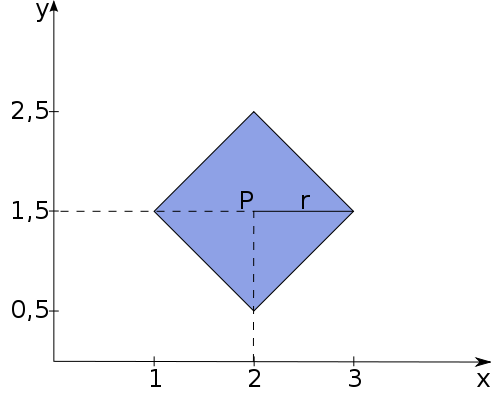
\includegraphics[width=8cm]{figuras/2D}}
		}{
			\Fonte{Wikipedia}			
		}	
	\end{figure}

\begin{alineascomponto}
\item Jogos 2.5D\\
Atribuído em jogos onde o 2D e o 3D são combinados para reproduzir um cenário mais realista. Nesta categoria os personagens são modelados em imagens 2D e se movimentam em um cenário 3D ou um personagem em 3D em um fundo 2D porém sendo mais comum um cenário que apresenta características de dimensão de profundidade a partir da sobreposição de imagens 2D.
Se divide na categorias: Isométrico, projeção oblíqua, \textit{billboarding} e escalamento do eixo Z.Na figura 9 é possível verificar a representação gráfica de um plano 2.5D (isométrico). 

\end{alineascomponto}

\begin{figure}[h!]
		\centering
		\Caption{\label{fig:exemplo-4}Representação gráfica de um espaço isométrico (2.5D)}	
		\UECEfig{}{
			\fbox{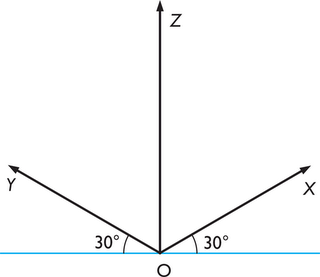
\includegraphics[width=8cm]{figuras/isometrico}}
		}{
			\Fonte{http://tittozamora.blogspot.com.br/2012/07/perspectiva-isometrica-decimo.html}			
		}	
	\end{figure}
	\pagebreak
\begin{alineascomponto}

\item Jogos 3D\\
São jogos onde o cenário é modelado tridimensionalmente sendo possível o personagem mover-se em qualquer direção.
Se dividem nas categorias
\begin{alineascomponto}
\item 3D Fixo - Jogo onde a câmera é fixa.
\item Primeira pessoa - Jogo onde a câmera está na posição na altura dos olhos do personagem.
\item Terceira pessoa - Jogo aonde câmera está próxima ao personagem, sempre o acompanhando. 
\end{alineascomponto}
Na figura 10 é possível verificar a representação gráfica de um plano 3D (tridimensional).
\end{alineascomponto}

\pagebreak
\begin{figure}[h!]
		\centering
		\Caption{\label{fig:exemplo-7}Representação gráfica de um espaço tridimensional}	
		\UECEfig{}{
			\fbox{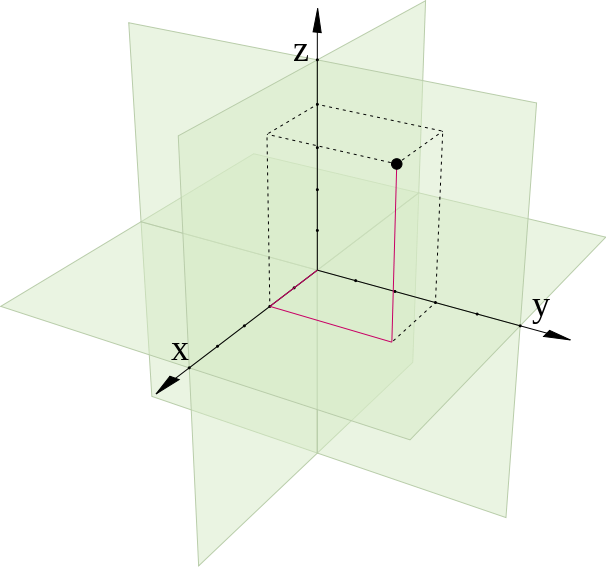
\includegraphics[width=8cm]{figuras/3D}}
		}{
			\Fonte{Wikipedia}			
		}	
	\end{figure}
	
\begin{comment}

http://www.dca.fee.unicamp.br/~martino/disciplinas/ia369/trabalhos/t3g1.pdf
https://pt.wikipedia.org/wiki/G%C3%AAneros_de_jogos_eletr%C3%B4nicos
\end{comment}
\section{Engenharia de Software}
\label{sec:engenharia-de-software}

Sommerville (2007) definiu engenharia de software como uma disciplina da engenharia que cuida de todos os aspectos da produção de software, desde a especificação do sistema até a sua manutenção, depois que ele entra em operação.

A engenharia é constituída de processos de software, que são conjuntos de atividades e resultados para se produzir um software. Existem quatro atividades fundamentais, são elas: 
\begin{alineascomponto}

\item Especificação de Software: o software a ser desenvolvido e as restrições para sua operação são definidos. 
Desenvolvimento de Software: o software deve ser feito atendendo suas especificações.
\item Validação de Software: o software tem de ser validado para garantir que está em cima do que o cliente deseja. 
\item Evolução do Software: o software sofre modificações para atender as necessidades do cliente.
\end{alineascomponto}

No desenvolvimento de software, o principal objetivo é a criação de sistemas que atendam às necessidades dos clientes e usuários, ou seja, uma correta especificação dos requisitos se torna essencial para que o desenvolvimento tenha sucesso. Uma forma de entender melhor esses requisitos é dividindo-os em: Requisitos Funcionais e Requisitos Não-Funcionais, Vasconcelos, Rouiller, Machado e Medeiros (2006).


Os Requisitos Funcionais definem as funções que componentes do sistema ou sistemas devem executar. 
Os Requisitos Não-Funcionais incluem limitações no produto, como por exemplo: desempenho, confiabilidade, segurança e limitações no desenvolvimento, como custos e tempo, componentes a serem reutilizados, entre outros.

\section{Desenvolvimento Mobile}
\label{sec:desenvolvimento-mobile}

Um dispositivo móvel pode ser definido como um computador de bolso, normalmente composto de uma tela e um teclado em miniatura podendo estes serem combinados em um so dispositivo conhecido como \textit{ touchscreen}.

Características dos dispositivos moveis:

\begin{alineascomponto}
 
\item Pequeno em tamanho
\item Baixo consumo de energia
\item Curto tempo de inicialização
\item Armazenamento de dados local e/ou remoto

	\end{alineascomponto}


Os dispositivos moveis mais populares são:

\begin{alineascomponto}
 
\item Smartphones
\item Tablets
\item Console portátil
\item Notebooks

	\end{alineascomponto}
	
	\begin{comment} 
	http://www.dca.fee.unicamp.br/~martino/disciplinas/ia369/trabalhos/t1g1.pdf

https://books.google.com.br/books?id=pWc3AgAAQBAJ&pg=PA46&lpg=PA46&dq=estilo+de+jogos+digitais&source=bl&ots=P8i8N4DcJL&sig=uj-5ewjDs8v_Ea5XAtmdELqSQMY&hl=pt-BR&sa=X&ved=0ahUKEwj85cSisLvJAhWON5AKHXH-CAEQ6AEIWDAJ#v=onepage&q=estilo%20de%20jogos%20digitais&f=false
\end{comment}

Toda esta tecnologia que possibilita a existência dos dispositivos moveis começou a partir do primeiro celular inventado, em 3 de abril de 1983, o Motorola DynaTAC 8000x. Foi então que em 1992 a empresa Apple lançou no mercado o primeiro PDA que continha memoria de 1MB e tela sensível ao toque, desde então esta tecnologia tem se desenvolvido e mostrado como
vantagem  a possibilidade dos dados serem acessados em qualquer lugar a qualquer hora.

Dentre os dispositivos moveis citados, o que mais se destacam são os \textit{smartphones}. Um \textit{smartphone} (telefone inteligente) poder ser definido como um celular que possui muitas funções. Essas funções são realizadas de maneira mais eficientes do que um celular normal, em geral possuem internet wiFi, navegadores, é possível realizar a instalação de aplicativos e possui um Sistema Operacional (SO). 

Uma das grandes vantagens dos \textit{smartphones} é a capacidade de qualquer pessoa desenvolver um aplicativo para o aparelho pois, em geral, o SO é um software aberto, onde existe a flexibilidade da criação de aplicativos.

Um Sistema Operacional é um conjunto de programas responsável por alocar recursos do hardware fornecendo também uma interface para o usuário. Os sistemas operacionais para smartphones mais conhecidos atualmente são: iOS, Android, Windows Mobile e BlackBerry

Segundo uma pesquisa realizada pela Gartner, o sistema operacional mais vendido em 2015 (para \textit{smartphones}) foi o Android e em segundo o iOS, conforme pode ser visto na figura 11.
\begin{figure}[h!]
		\centering
		\Caption{\label{fig:exemplo-1}Venda Mundial de Smartphones por Sistemas Operacionais}	
		\UECEfig{}{
			\fbox{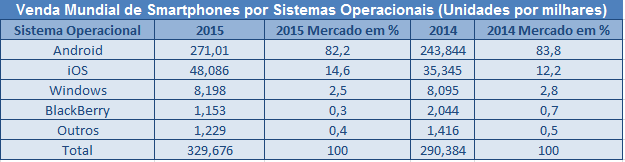
\includegraphics[width=13cm]{figuras/GartnetSamart}}
		}{
			\Fonte{Gartner, 2015}			
		}	
	\end{figure}

\subsection{Aplicativos Moveis}
Um aplicativo móvel, conhecido também como App é um software desenvolvido para dispositivos moveis, por exemplo, \textit{smartphones},  \textit{Tablets}, \textit{notebboks}, esses aplicativos podem ser nativos, Web ou híbridos.

\begin{alineascomponto}

\item Aplicativos Nativos

São os aplicativos que podem ser acessados na tela principal através de seu ícone. Podem ser instalados através de um aplicativo de loja especifico para sua plataforma, como por exemplo o sistema iOS utiliza a App Store baixar seus aplicativos,enquanto o Android utiliza o Google Play. Esses aplicativo nativos residem no dispositivo.

\item \textit{Mobile Web Apps}

São aplicativos que na verdade são sites e não aplicativos raiz, como os nativos. São executados a partir de um navegador e normalmente criado um ícone na tela principal do dispositivo para que quando clicando ele acesse a URL determinada.

\item Aplicativos Híbridos

São os aplicativos que são parcialmente web e nativos.
Estes devem ser baixados pela loja de aplicativos, ficam armazenados no dispositivo porém podem também serem utilizado como web App.

	\end{alineascomponto}
	
Segundo dados divulgados pelo Ministério de Ciência, Tecnologia e Inovação (MCTI) o mercado de aplicativos moveis está em alta, movimentando mais de US\$ 25 bilhões por ano no Brasil, com expectativas de alcançar US\$ 70 milhões até 2017.
	
	
	\begin{comment}
http://www.luisaambros.com/blog/diferenca-entre-aplicativos-nativos-hibridos-e-mobile-web-apps/

http://www.correiobraziliense.com.br/app/noticia/tecnologia/2015/05/11/interna_tecnologia,482694/brasil-decola-na-industria-de-apps-e-mercado-acumula-lucros-nesta-deca.shtml
\end{comment}
	
\begin{comment}
http://www.telefonescelulares.com.br/o-que-e-smartphone/
http://pt.slideshare.net/cetorres/palestra-mobilidade-computao-mvel-dispositivos-e-aplicativos-2013
\end{comment}

\section{Android}
\label{sec:Android}
Android é um sistema operacional para dispositivos moveis, seu código é aberto (\textit{open-source}).
Inicialmente desenvolvido pela Android Inc, em 2003 compradra pela empresa Google e desde 2007 mantida pela \textit{Open Handset Alliance} (OHA).

O sistema operacional Android possui seu núcleo (\textit{Kernel}) em Linux e utiliza Java como linguagem de programação padrão. Também utiliza de sua propia maquina virtual chamada de Dalvik.


A maquina virtual Dalvik possui grande diferença entre a Java Virtual Machine (JVM) o que faz seu desenho seja bem superior; a Dalvika é baseada em registradores e não em pilhas como a JVM.


A Dalvika executa seus arquivos na extensão ".dex" (Dalvik Executable) que nada mais são do que arquivos Java já previamente projetados e compilados realizando a otimização de memoria e compartilhamento de dados.


Na figura 12 é possivel fazer um comparativo entre a JVM (.class) e a Dalvik VM (.dex).

	\begin{figure}[h!]
		\centering
		\Caption{\label{fig:exemplo-2}Comparação do formato .class da JVM com o .dex usado pela Dalvik VM.}	
		\UECEfig{}{
			\fbox{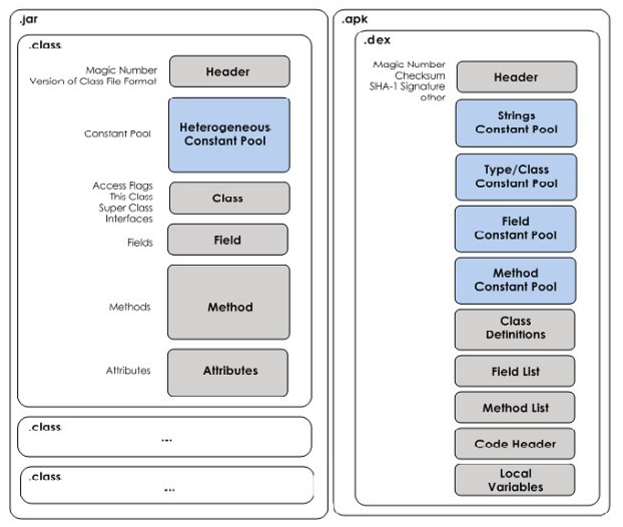
\includegraphics[width=13cm]{figuras/JvmDvm}}
		}{
			\Fonte{Google Imagens}			
		}	
	\end{figure}

\subsection{Google Play }

Google Play também conhecida como Google Play Store é a loja virtual da Google para venda de aplicativos. Antigamente esta loja virtual recebia o nome de Android Market mas em 2002 seu nome mudou para haver a unificação de produtos.
No Google Play esta disponível para usuário baixar aplicativos gratuito e/ou pagos.

\begin{comment}http://smartmundo.com/o-que-e-play-store/
\end{comment}
Para um desenvolvedor distribuir seus aplicativos na Google Play é necessario que o mesmo faça seu cadastro e pague uma quantia de U\$25,00, feito isso
sera possível fornecer seu aplicativo na loja virtual.
Um vez que o desenvolvedor tem a conta criada é possível ter acesso a comentários, estatísticas e erros de seus aplicativos. Caso o aplicativo seja pago, o lucro para o desenvolvedor é de 70\% do valor cobrado pelo aplicativo.
\begin{comment}http://www.tutoriandroid.com/2012/05/como-publicar-no-google-play.html
\end{comment}

\subsection{Versões Disponíveis}

Desde de seu inicio, o Android nomeia suas versões com nomes de doces e sobremesas e seguem uma ordem alfabética.
Ainda não foi revelada pela empresa o real motivo deste padrão de nomenclatura porém foi bem aceita pelo o publico.
Atualmente existem 13 versões do sistema operacional Android, estas apresentados na tabela 1.

\begin{comment}
http://www.aplicativosandroid.com/conhecam-todas-as-versoes-do-android-e-seus-maravilhos-doces/3891 ---  e tabela ----- http://www.tecmundo.com.br/android/82344-linha-tempo-dentro-evolucao-do-sistema-android.htm
\end{comment}


\begin{table}[h!]
	\Caption{\label{tabela-android} Tabela contendo nome, versão e ano de lançamento dos sitemas Androids.}%
	\IBGEtab{}{%
		\begin{tabular}{ccc}
			\toprule
			Nome & Versões & Ano de Lançamento \\
			\midrule \midrule
			Alpha (Apple Pie)  & 1.0 & 2008 
			\\
			Beta (Banana Bread) & 1.1 & 2009 \\
			Cupcake & 1.5 & 2009\\
			Donut & 1.6 & 2009 \\
			Eclair & 2.0 e 2.1 & 2009 \\
			Froyo & 2.2 & 2010 \\
			Gingerbread & 2.3 & 2010 \\
			Honeycomb & 3.0; 3.1; 3.2 & 2011 \\
			Ice Cream Sandwich & 4.0 & 2011 \\
			Jelly Bean & 4.1; 4.2; 4.3 & 2012 e 2013 \\
			KitKat & 4.4 & 2013 e 2014 \\
			Lollipop & 5.0 & 2014 e 2015 \\
			Marshmallow & 6.0 & 2015 \\
			\bottomrule
		\end{tabular}%
	}{%
	\Fonte{TecMundo, 2015}%
	
}
\end{table}
\pagebreak
\section{Scrum}
\label{sec:scrum}

Scrum é uma metodologia ágil para gestão e planejamento de projetos de softwares e sua base fundamental pode ser bem descrita na figura 13.

	\begin{figure}[h!]
		\centering
		\Caption{\label{fig:exemplo}Prática do Scrum}	
		\UECEfig{}{
			\fbox{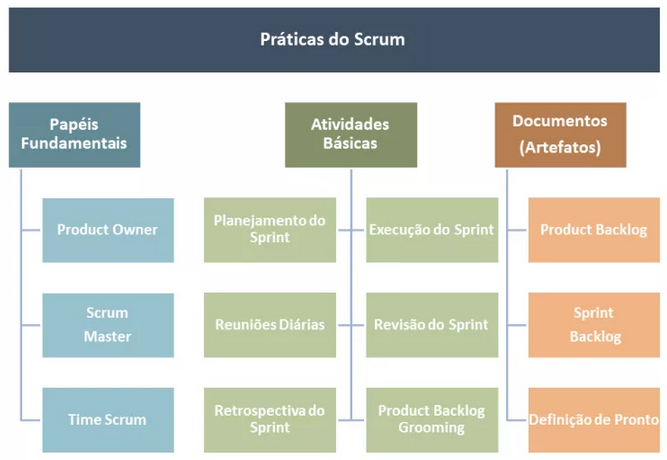
\includegraphics[width=10cm]{figuras/PraticaScrum}}
		}{
			\Fonte{MindMaster, 2014}			
		}	
	\end{figure}

Cada equipe de Scrum, geralmente, possuem 3 papeis:
\begin{alineascomponto}
	\item \textit{Product Owner}
	
É responsável por decidir os recursos e funcionalidades utilizadas no projeto é também sua responsabilidade manter clareza no objetivo do projeto, para que haja uma melhor interação o ProductOwner geralmente colabora com o ScrumMaster.

	\item \textit{Scrum Master}
	
É de sua responsabilidade ajudar todos envolvidos a entender os valores, princípios e práticas do Scrum. Também fica responsável por melhorias no uso do Scrum e está sempre orientando para que não haja a perda de foco. 

	\item \textit{Development Team}
	
São todos da equipe responsáveis pelo desenvolvimento em si do software, possuem papeis como: arquiteto, testador, programador entre outros. Para esta equipe é recomendável que se organizem para determinar a melhor maneira de realizar o trabalho.

	\end{alineascomponto}
	
		A figura 14 representa o processo de interação das atividades.

	\begin{figure}[h!]
		\centering
		\Caption{\label{fig:exemplo-3} Interação das atividades }	
		\UECEfig{}{
			\fbox{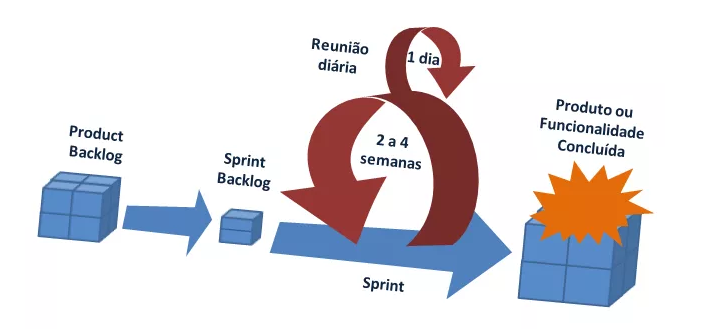
\includegraphics[width=10cm]{figuras/InteracaoScrum}}
		}{
		\Fonte{MindMaster, 2014}			
	}	
	\end{figure}
	
O \textit{Product Owner} tem a visão final do produto, representado na figura como grande cubo. Este cubo é "divido" em vários outros cubos pequenos, este chamado de \textit{Product Backlog}.

O \textit{Product Backlog} pode ser descrito, em uma forma simplificada, como pequenas etapas/objetivos para se chegar ao produto final.
Para planejar a prioridade dos \textit{Backloge} também quando e quanto tempo durará seu desenvolvimento, é utilizado o \textit{Sprint}.

O \textit{Sprint} tem duração mediana de 2 a 4 semanas, mas é também flexível dependendo do tempo desenvolvimento final estimado no começo do planejamento.

Também existe a técnica do \textit{Daily Scrum}, utilizado para o desenvolvimento deste jogo junto a sua monografia. Para o \textit{Daily Scrum}, é utilizado as três perguntas consideradas básicas para haver um melhor desenvolvimento de todos da equipe.
Estas são:

\begin{enumerate}
   \item O que fiz ontem que ajudou o time a atingir a meta do \textit{Sprint}?
   \item O que vou fazer hoje para ajudar o time a atingir a meta do \textit{Sprint}?
   \item  Existe algum impedimento que não permita a mim ou ao time atingir a meta do \textit{Sprint}?
 \end{enumerate}
 
Para a utilização do método Scrum há várias outras técnicas existentes, porém devido ao tempo curto e a quantidade de integrantes dispostos no desenvolvimento do jogo Caapora, foi somente utilizado os métodos acima.

\section{Controle de Versão}
\label{sec:Controle-de-Versão}

O controle de versão tem como objetivo a gerencia de versões de um mesmo projeto. Vários programadores podem trabalhar em um mesmo projeto sendo possível manter um histórico de atualizações.

Dentre as infinidades de vantagens para se utilizar um "controlador de versões" as três principais que se destacam são:
\begin{alineascomponto}
	
   \item Possibilidade de salvar o histórico
   \item Possibilidade de desenvolver versões diferentes
   \item Possibilidade de se programar em paralelo

	\end{alineascomponto}
	
	
O controle de versão funciona da seguinte forma: os históricos contendo as modificações de cada versão ficam armazenados em um repositório (servidor). Este processo dá à liberdade para que o desenvolvedor possa baixar a última versão, trabalhar em seu código e posteriormente atualizar a versão já previamente armazenada no servidor, este processo pode ser visto na figura 15.

	\begin{figure}[h!]
		\centering
		\Caption{\label{fig:exemplo-4} Funcionamento do Controle de Versão}	
		\UECEfig{}{
			\fbox{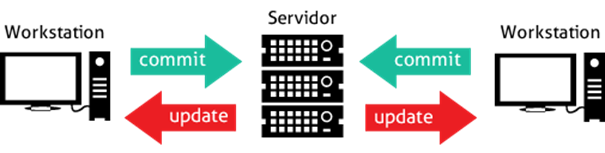
\includegraphics[width=13cm]{figuras/ControleVersao}}
		}{
		\Fonte{AprendendoWWW, 2015}			
	}	
	\end{figure}
	
	Para que seja realizada a sincronização entre a \textit{workstation} e o servidor é necessário utilizar os comandos:
	
	\begin{alineascomponto}
\item \textit{Commit} - realiza o envio das alterações realizadas para o servidor gerando um novo histórico de atualizações.
\item \textit{Update} - realiza o envio da última versão contida no servidor para a \textit{workstation}.

	\end{alineascomponto}
	
	\subsection{Bitbucket}
	
No mercado atualmente existem dois grandes serviços que disponibilizam o controle de versionamento e estes são: Github e o Bitbucket.

O escolhido para desenvolvimento do Caapora games foi o Bitbucket, e é uma ferramente de domínio da empresa Atlassian e implementa dois padrões de versionamentos, o GIT e o Mercurial.


A equipe optou por utilizar este tipo de tecnologia para que houvesse uma melhor interação entre os membros e para que o desenvolvimento ocorresse simultaneamente e o
versionamento utilizado é o GIT.

\section{Inteligência Artificial}
\label{sec:inteligencia-artificial}

A Inteligência Artificial (IA) é um ramo de pesquisa da ciência da computação que procura através de meio computacionais desenvolver mecanismos e/ou dispositivos que simulem a capacidade do ser humano de raciocinar e resolver problemas, ou seja, ser inteligente. 

O campo de IA tem como objetivo, o contínuo aumento da "inteligência"  do computador, pesquisando, para isto, os fenômenos da inteligência natural. Para este fim, IA é definida  como sendo uma coleção de técnicas suportadas por computador emulando algumas capacidades dos seres humanos. Esta coleção inclui:

\begin{alineascomponto}
	
   \item Resolução de problemas
   \item Compreensão de Linguagem Natural
   \item Visão e Robótica
   \item Sistemas Especialistas e Aquisição de Conhecimento
   \item Metodologias de Representação de Conhecimento

	\end{alineascomponto}
	
Hoje em dia a Inteligência Artificial é utilizada em vários fins, não só exclusivamente para informática e um dos pontos em que se destaca é para o desenvolvimento de jogos. 

Primeiramente utilizada em jogos clássicos como xadrez ou jogo da velha e atualmente utilizada para jogos digitais.


Os algoritmos de IA desenvolvidos para jogos digitais podem ser divididos em três blocos:

\begin{alineascomponto}
	
\item Movimento:

De como um personagem é movimentado, do local de inicial ate o destino final, também determina o calculo do percurso, detectando objetos e desviando de obstáculos.
   
 \item Tomada de Decisão:
 
Cada personagem possui um conjunto de atividades e estados possíveis, estes sendo: estar parado, fugir, atacar adversário entre outros. Para que cada ação seja possível, a personagem precisara fazer uma tomada de decisão analisando o contexto. Esta decisão pode ser de ativar um algoritmo de movimento, alterar um estado interno ou a animação. Não necessariamente essas alterações serão visuais.

\item Estratégia:

A maioria dos jogos digitais desenvolvidos com IA ocorrem nos dois tipos já citados estes também podem conter personagens que trabalham em grupo ou equipe contando com uma tomada de decisão individual.

	\end{alineascomponto}

	
As pesquisas iniciaram-se na Segunda Guerra Mundial com os cientistas Hebert Simon, Allen Newell,  Jonh McCarthy com o objetivo em comum de reproduzir uma maquina que simulasse o cérebro humano. (SANTOS,2015) 

\section{Busca Heurística}
\label{sec:Busca-Heurística}

A busca heurística pode ser definida como uma estrategia que faz uso do conhecimento especifico do problema, sendo possível obter soluções mais eficientes do que uma estratégia sem informação. 0Russel e Norvig (2003).

De acordo com Rich e Knight (1993), heuristca é uma técnica eficiente para um processo de busca. A heurística, mesmo que as vezes possa passar por pontos de interesse despercebidos pode levar a direcionamentos interessantes. A heurística aprimora os caminhos a serem percorridos, entretanto pode desconsiderar o melhorar caminho a percorrer. 

Dentre as diversas heurísticas existentes, a que se destacou e mostrou melhor performance para o jogo Caapora foi o algoritmo A*
	

\subsection{Algoritmo A* (A estrela)}	
O A* (lê-se A estrela) é um algoritmo de busca de caminho \textit{(pathfinding)}. Segundo Russel (2003) A* é a forma mais eficiente pela busca da melhor escolha na qual avalia os nós combinando o custo para alcançar cada nó \textit{g(n)} e o custo do nó ate o objetivo h(n).

	\begin{equation}
		\begin{aligned}
		\textbf{ f(n) = g(n) + h(n)} 
		\end{aligned}
	\end{equation}
 
A função \textit{f(n)} representa o custo estimado da solução menos custosa passando por \textit{n} e chegando ao estado-objetivo. O A* utiliza também o método de lista aberta e fechada aonde listas abertas armazenam todos o nós que foram gerados porém ainda não examinados e a fechada armazena os nós que já analisados.

O algoritmo A* é completo e eficiente contanto que a função heurística \textit{f(n)} não superestime o custo ate o estado-objetivo.

\begin{comment}
http://dsc.inf.furb.br/arquivos/tccs/monografias/2005-1jeanitabassanidasilvavf.pdf
file:///C:/Users/Talita/Downloads/601-1351-2-PB.pdf
\end{comment}

\section{Orientação Objeto}
\label{sec:orientação-objeto}	

O paradigma orientado a objeto busca representar o universo de desenvolvimento de software como o mundo real de forma a evitar reutilização de código, abstração de código, maior facilidade de leitura do código.

\subsection{Classes e Objetos}	
As classes representam uma forma de um grupo de objetos definindo como serão seus comportamentos e características antes de criá-lo (instanciar)


\subsection{Classes Abstratas}	
Uma classe abstrada define características e comportamentos comuns a um conjunto de classes de forma a tornar o código mais escalável e evitar repetição de código.

\subsection{Interface}	
Interface é um recurso da orientação a objetos que permite criamos uma aplicação com um maior nível de abstração, definindo comportamentos que deverão ser obrigatórios para as classes que implementarão uma interface definida.


\subsection{Padrões de Projeto}	
Padrões de projetos são soluções padronizadas que buscam resolver problemas comuns frequentes que se apresenta em projetos orientadas a objetos.


\subsection{Singleton}	
Padrão de projeto criacional que garante uma única instancia para um objeto de uma determinada classe. Exemplos do uso deste modelo são nas Classes Player e GameManager que podem ter uma única instancia durante todo o jogo.


\subsection{Object Pool}	
Padrão de projeto criacional que permite alocar um grupo de objetos em uma estrutura para posterior uso sobre demanda. No game foi utilizado para armazenar objetos do tipo fogo que seriam que ser multiplicados durante o jogo dando um efeito de expansão das chamas.